\documentclass[times]{article}

\usepackage[margin=1.0in]{geometry}
\usepackage{graphicx}
\usepackage{adjustbox}
\usepackage{float}
\usepackage{placeins}
\usepackage[none]{hyphenat}
\usepackage{amsmath}
\usepackage[us]{datetime}
\usepackage[explicit]{titlesec}
\usepackage{standalone}
\maxdeadcycles=100000
\begin{document}
	\title{”COMP SCI 5401 FS2017 Assignment 2c}
	\author{Dalton Cole \\ drcgy5@mst.edu}
	\date{\formatdate{3}{12}{2017}}
	\maketitle

	\section{Methodology}
	For this experiment, a coevolutionary search of the Iterated Prisoner’s Dilemma was performed. Table \ref{tab:config} shows the configurable parameters for the experiment. For the statistical analysis shown later in this report, Table \ref{tab:this_config} shows the configuration parameters used. 

	The following sub-sections will describe some of the underlining structures of the coevolutionary algorithm used.

	\subsection{Initial Starting Population}
	The fitness for the initial starting population was assigned via the tic-for-tat method. This only influenced in the parent selection portion of first evaluation cycle. The purpose of this is because the underlining goal is to create an evolutionary algorithm which is strong against the tic-for-tat method. Having the initial population be based on that gives the tic-for-tat initial goal.

	\subsection{Move Queue}
	Every Prisoner initially starts out with the exact same move queue each time it is evaluated. This is done so each strategy is on an even playing field, meaning, no strategy has an easier or harder move sequence to evolve from.

	\subsection{Tree Generation}
	There is a fifty-fifty percent chance that full method or grow method for ramped half-and-half will be chosen. When grow method is chosen, each node has a $((Max Depth - Current Depth) / Max Depth) * 100$ percent chance of growing into a branch. Each operator and memory location has an equal chance of being chosen. 

	\subsection{Sub-Tree Crossover}
	For recombination, sub-tree crossover was used. A node of equal depth on each tree was chosen to switch between one another. An equal depth node was chosen as to not go over the depth limit.

	\begin{table}
		\centering
		\caption{Configurable Parameters}
		\label{tab:config}
		\begin{tabular}{| c | c |}
			\hline
				\textbf{Parameter} & \textbf{Options} \\
				\hline
				Random Seed & Any Integer \\
				\hline
				Number of Iterations to Play & Any Integer \\
				\hline
				Number of Iterations to Keep in Memory & Any Integer \\
				\hline
				Maximum Tree Depth & Any Integer \\
				\hline
				Number of Runs & Any Integer \\
				\hline
				Number of Fitness Evaluations & Any Integer \\
				\hline
				Population Size & Any Integer \\
				\hline
				Number of Children Per Generation & Any Integer \\
				\hline
				Parent Selection Strategy 	& Fitness Proportional Selection \\
											& Over Selection \\
				\hline
				Survival Selection	& Truncation \\
									& K-Tournament without Replacement \\
				\hline
				Parsimony Pressure Penalty Coefficient & Any Float \\
				\hline
				Termination Convergence Criterion & Any Integer \\
				\hline
				Survival Selection Strategy 	& Plus \\
												& Comma \\
				\hline
				Coevolutionary Fitness Sampling	& Any Integer between 1 and Population Size + Children Count - 1 \\
				\hline
				Detect Cycling & true or false \\
				\hline
				Deter Cycling & true or false \\
			\hline
		\end{tabular}
	\end{table}

	\begin{table}
		\centering
		\caption{Configurable Parameters}
		\label{tab:this_config}
		\begin{tabular}{| c | c |}
			\hline
			\textbf{Parameter} & \textbf{Options} \\
			\hline
			Random Seed & 0, 1, 2 \\
			\hline
			Number of Iterations to Play & 30 \\
			\hline
			Number of Iterations to Keep in Memory & 5 \\
			\hline
			Maximum Tree Depth & 10 \\
			\hline
			Number of Runs & 30 \\
			\hline
			Number of Fitness Evaluations & 10,000 \\
			\hline
			Population Size & 100 \\
			\hline
			Number of Children Per Generation & 50 \\
			\hline
			Parent Selection Strategy 	& Fitness Proportional Selection \\
			\hline
			Survival Selection	& Truncation \\
			\hline
			Parsimony Pressure Penalty Coefficient & 0.0, 0.5, 1.0 \\
			\hline
			Termination Convergence Criterion & 10,000 \\
			\hline
			Survival Selection Strategy 	& Plus \\
			\hline
			Coevolutionary Fitness Sampling	& 10 \\
			\hline
			Detect Cycling & false \\
			\hline
			Deter Cycling & false \\
			\hline
		\end{tabular}
	\end{table}


	\section{Experimental Setup}
	Table \ref{tab:this_config} shows the configurations used for this experiment. One hundred was used as the population size so the experiment would run in a timely manner. Fifty children was chosen as a happy balance between exploitation and exploration. Fitness Proportional Selection was selected because it gave a slight speed boost when compared to K-Tournament without Replacement. The Plus Survival Selection Strategy was selected so past generations could more directly influence current generations in the creation of a more optimal solution. A Coevolutionary Fitness Sampling value of 10 was chosen because it lead to more generations than a larger value, but comparing strategies to one another is still seen as important. Parsimony Pressure was selected to test how much it effected the dependent variable (absolute fitness against Tic-For-Tat). Parsimony Pressure took on three different values over the course of the experiment: 0.0, 0.5, and 1.0.

	\section{Results}

	The results of the experiment showed that there was no significant difference between using a higher Parsimony Pressure Penalty Coefficient when compared to a lower one or none at all. Figures \ref{fig:stat_rel_01}, \ref{fig:stat_rel_02}, \ref{fig:stat_rel_12}, and \ref{fig:stat_abs_012} all come to this conclusion. It is worth noting, as seen in Table \ref{tab:std_mean}, that the mean fitness increases as parsimony pressure goes up, just not at a significant level.

	Figures \ref{fig:relative_plot_0}, \ref{fig:relative_plot_1}, and \ref{fig:relative_plot_2} show the relative fitness plots for the three trials. Figures \ref{fig:absolute_plot_0}, \ref{fig:absolute_plot_1}, and \ref{fig:absolute_plot_2} show the absolute fitness plots for the three trials.

	\section{Discussion}

	Figures \ref{fig:relative_plot_0}, \ref{fig:relative_plot_1}, and \ref{fig:relative_plot_2} shows the relative progression of fitness value between coevolutionary algorithms. All three of these figures show a decrease in best fitness over time. This is likely because Prisoners are becoming better at playing against one another. Figure \ref{fig:relative_plot_0} has a general decrease in average fitness, while the figures with a non-zero parsimony pressure have a slow increase in average fitness. This may be because fitness is initially decreased due to the parsimony pressure, and increases as large trees become sparse. None of th

	Figures \ref{fig:absolute_plot_0}, \ref{fig:absolute_plot_1}, and \ref{fig:absolute_plot_2} shows the absolute progression of fitness value between coevolutionary algorithms. All the algorithms have a near perfect fitness against tic-for-tat, if not perfect. Although not significantly different, having a parsimony pressure does result in an optimal fitness vs not having parsimony pressure. The average absolute fitness for each three algorithms seem to be rather stable.


	Figures \ref{fig:stat_rel_01}, \ref{fig:stat_rel_02}, \ref{fig:stat_rel_12}, \ref{fig:stat_abs_012} show no significant difference between any of the parsimony pressure values. Figure \ref{tab:std_mean} does however show that the mean value generally increases as parsimony pressure increases.

	\section{Conclusion}

	From this experiment, it has been found that although a higher parsimony pressure coefficient leads to a higher mean fitness, there is no significant difference between using no parsimony pressure and using a medium or high coefficient. In the future it is worth looking at what effects on fitness re-introducing assigning fitnesses based on tic-for-tat every $x$ generations will have on the end fitness.

	\begin{figure}
		\caption{Relative Fitness For Parsimony Pressure Penalty Coefficient = 0.0}
		\label{fig:relative_plot_0}
		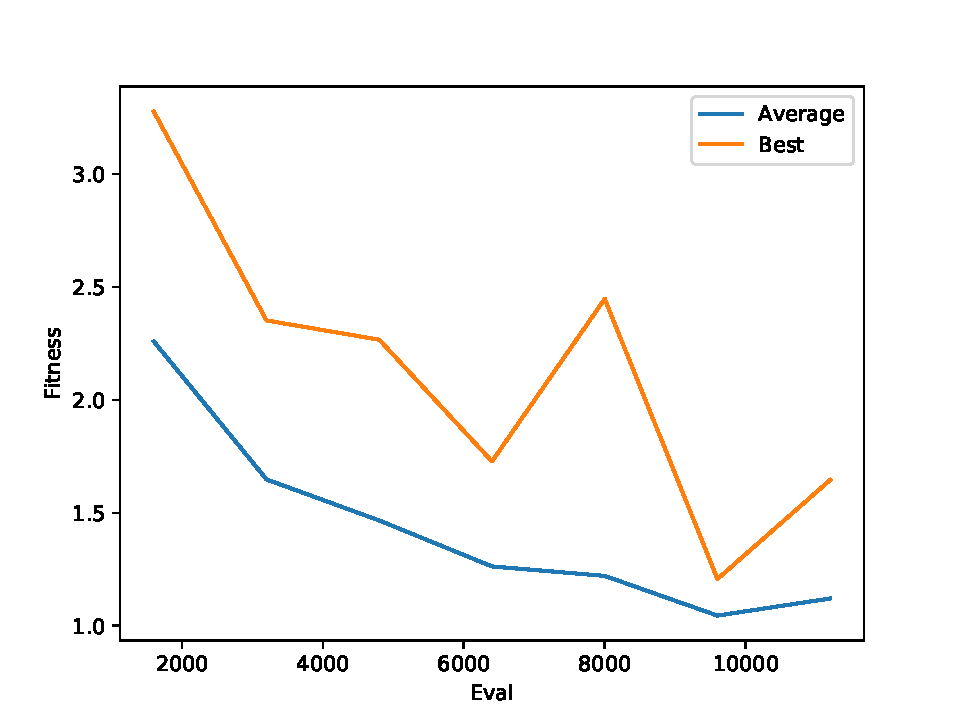
\includegraphics[width=\textwidth]{../graph/graphs/0.pdf}
	\end{figure}

	\begin{figure}
		\caption{Relative Fitness For Parsimony Pressure Penalty Coefficient = 0.5}
		\label{fig:relative_plot_1}
		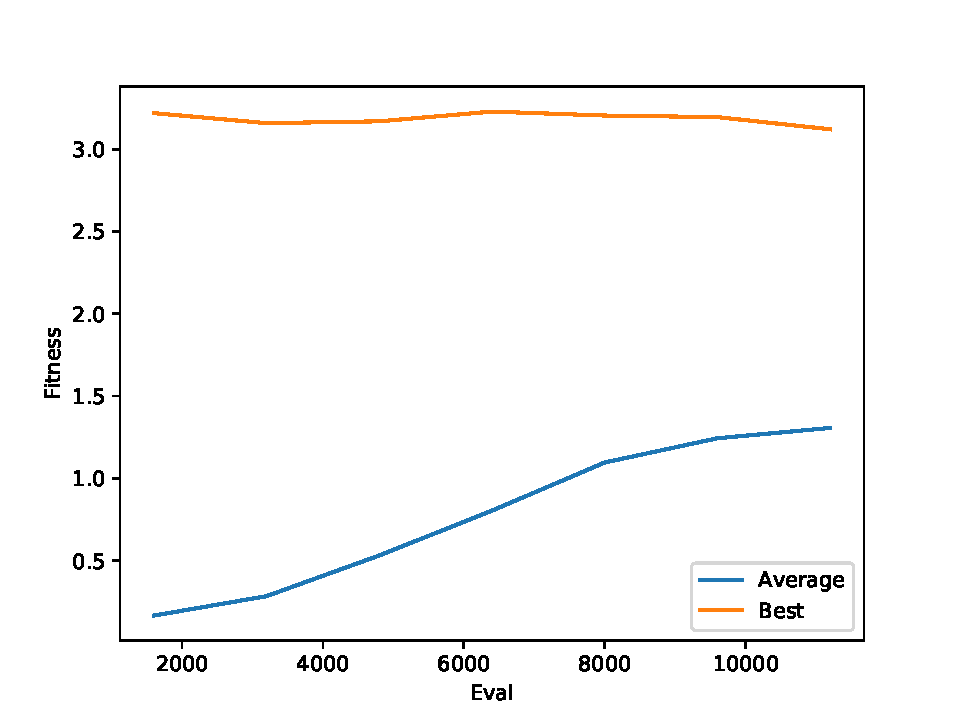
\includegraphics[width=\textwidth]{../graph/graphs/1.pdf}
	\end{figure}

	\begin{figure}
		\caption{Relative Fitness For Parsimony Pressure Penalty Coefficient = 1.0}
		\label{fig:relative_plot_2}
		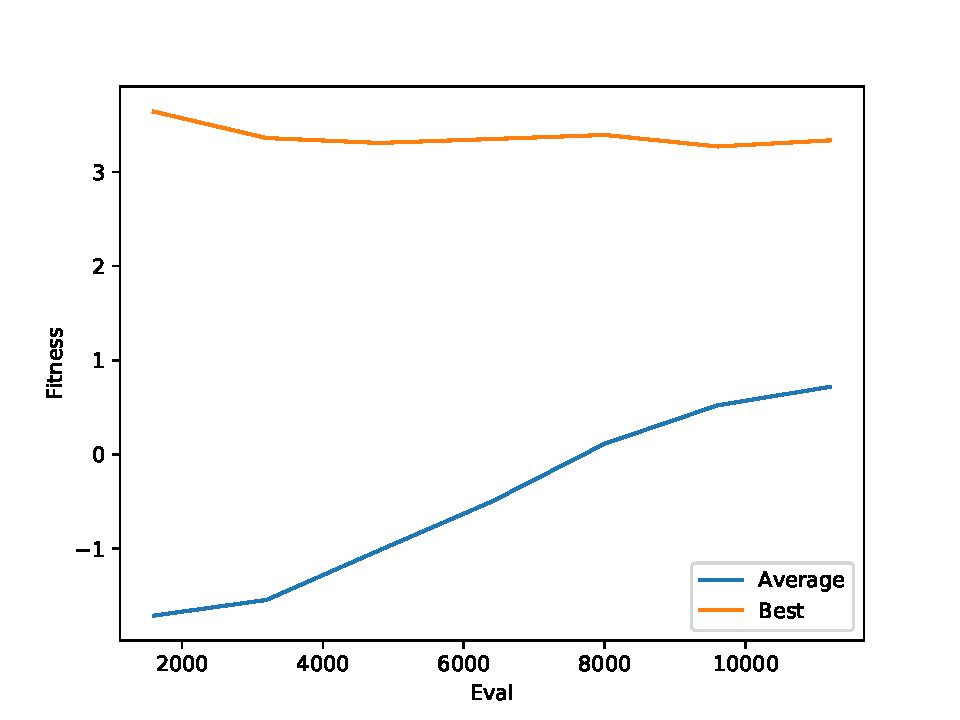
\includegraphics[width=\textwidth]{../graph/graphs/2.pdf}
	\end{figure}


	\begin{figure}
		\caption{Absolute Fitness For Parsimony Pressure Penalty Coefficient = 0.0}
		\label{fig:absolute_plot_0}
		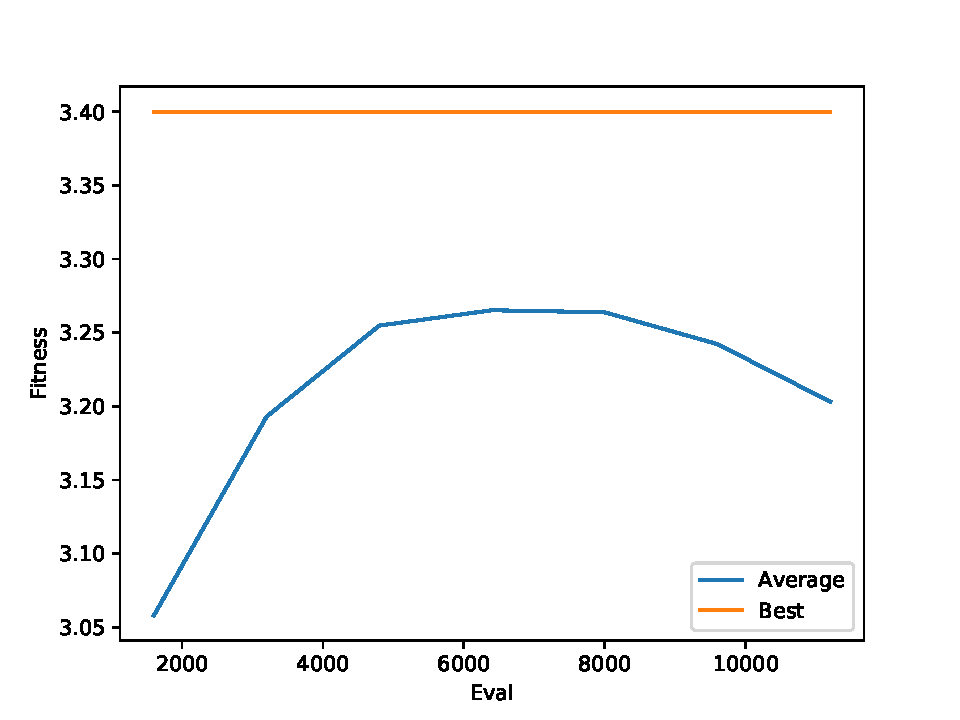
\includegraphics[width=\textwidth]{../graph/absolute/0.pdf}
	\end{figure}

	\begin{figure}
		\caption{Absolute Fitness For Parsimony Pressure Penalty Coefficient = 0.5}
		\label{fig:absolute_plot_1}
		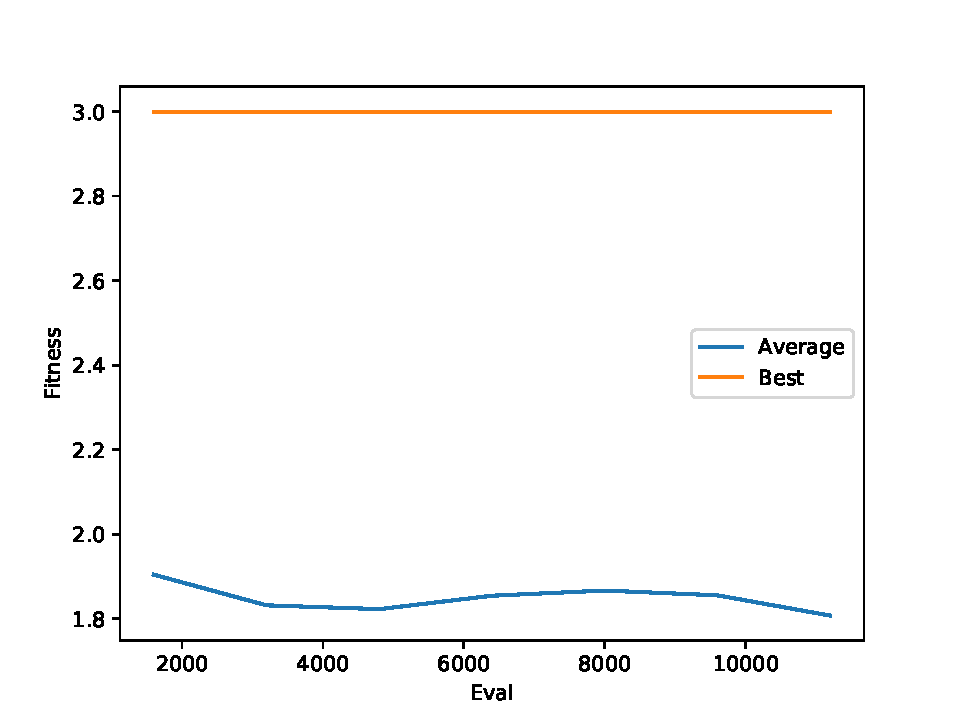
\includegraphics[width=\textwidth]{../graph/absolute/1.pdf}
	\end{figure}

	\begin{figure}
		\caption{Absolute Fitness For Parsimony Pressure Penalty Coefficient = 1.0}
		\label{fig:absolute_plot_2}
		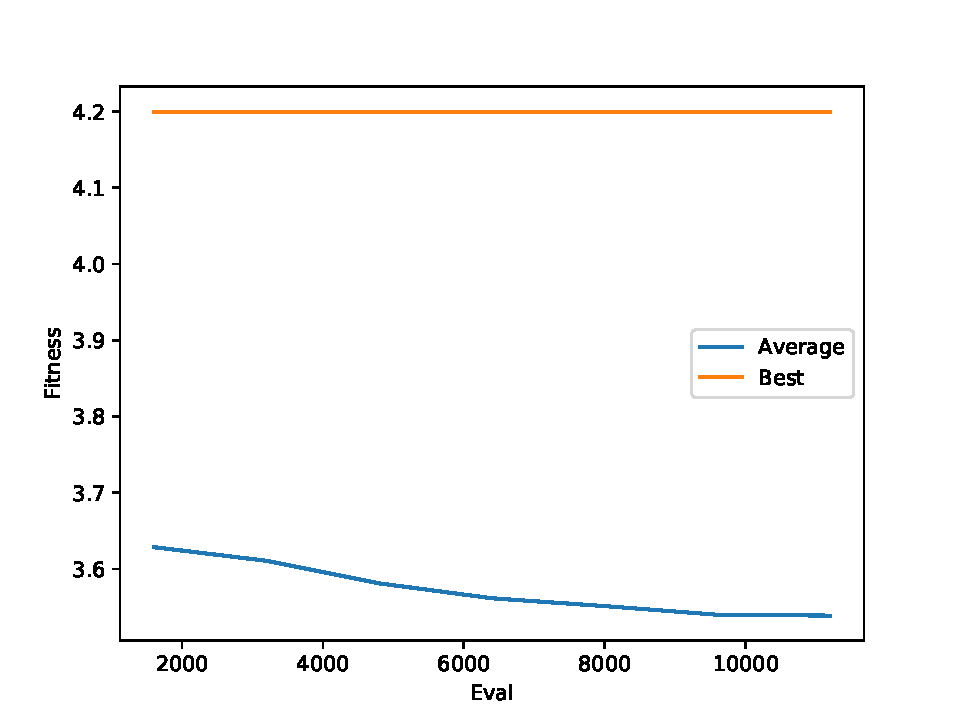
\includegraphics[width=\textwidth]{../graph/absolute/2.pdf}
	\end{figure}

	\begin{figure}
		\caption{Statistical Analysis for Relative Parsimony Pressure Penalty Coefficient 0.0 VS 0.5}
		\label{fig:stat_rel_01}
		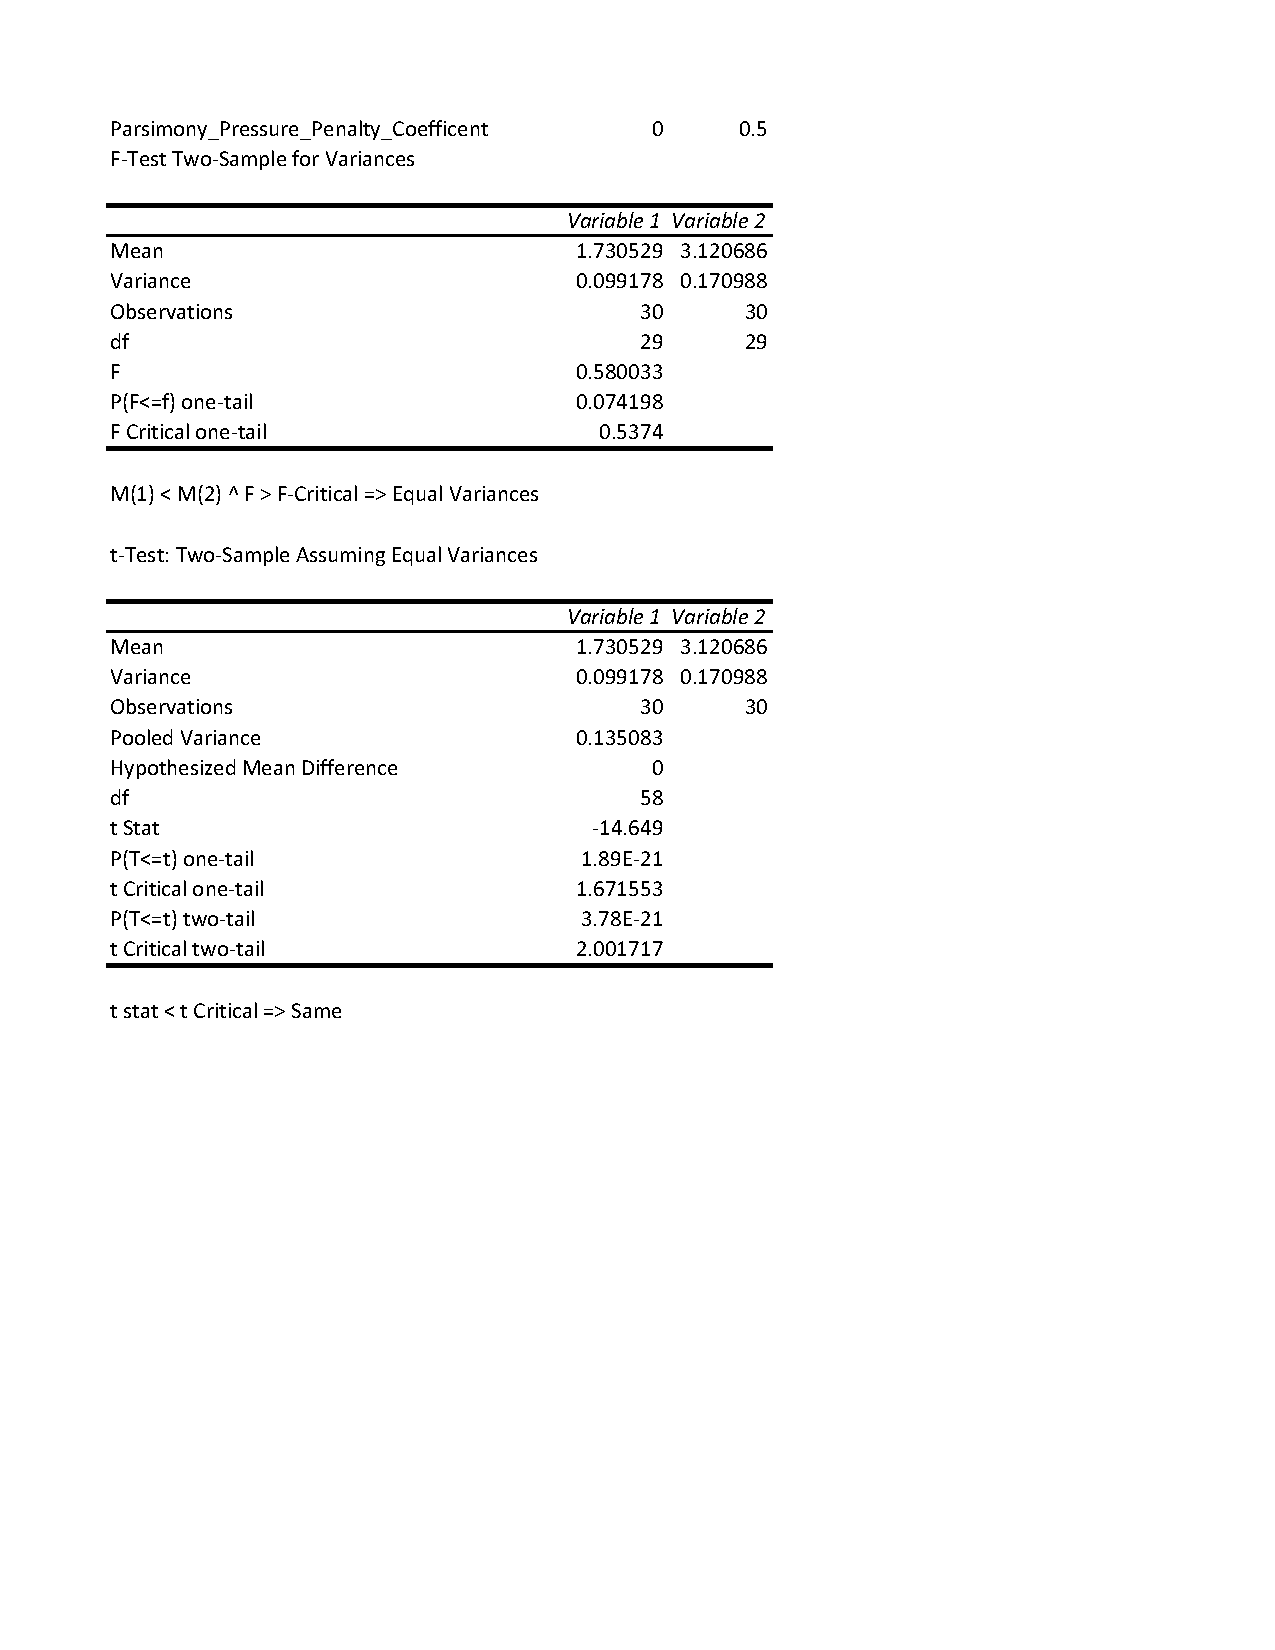
\includegraphics[width=\textwidth]{./pictures/relative_01.pdf}
	\end{figure}

	\begin{figure}
		\caption{Statistical Analysis for Relative Parsimony Pressure Penalty Coefficient 0.0 VS 1.0}
		\label{fig:stat_rel_02}
		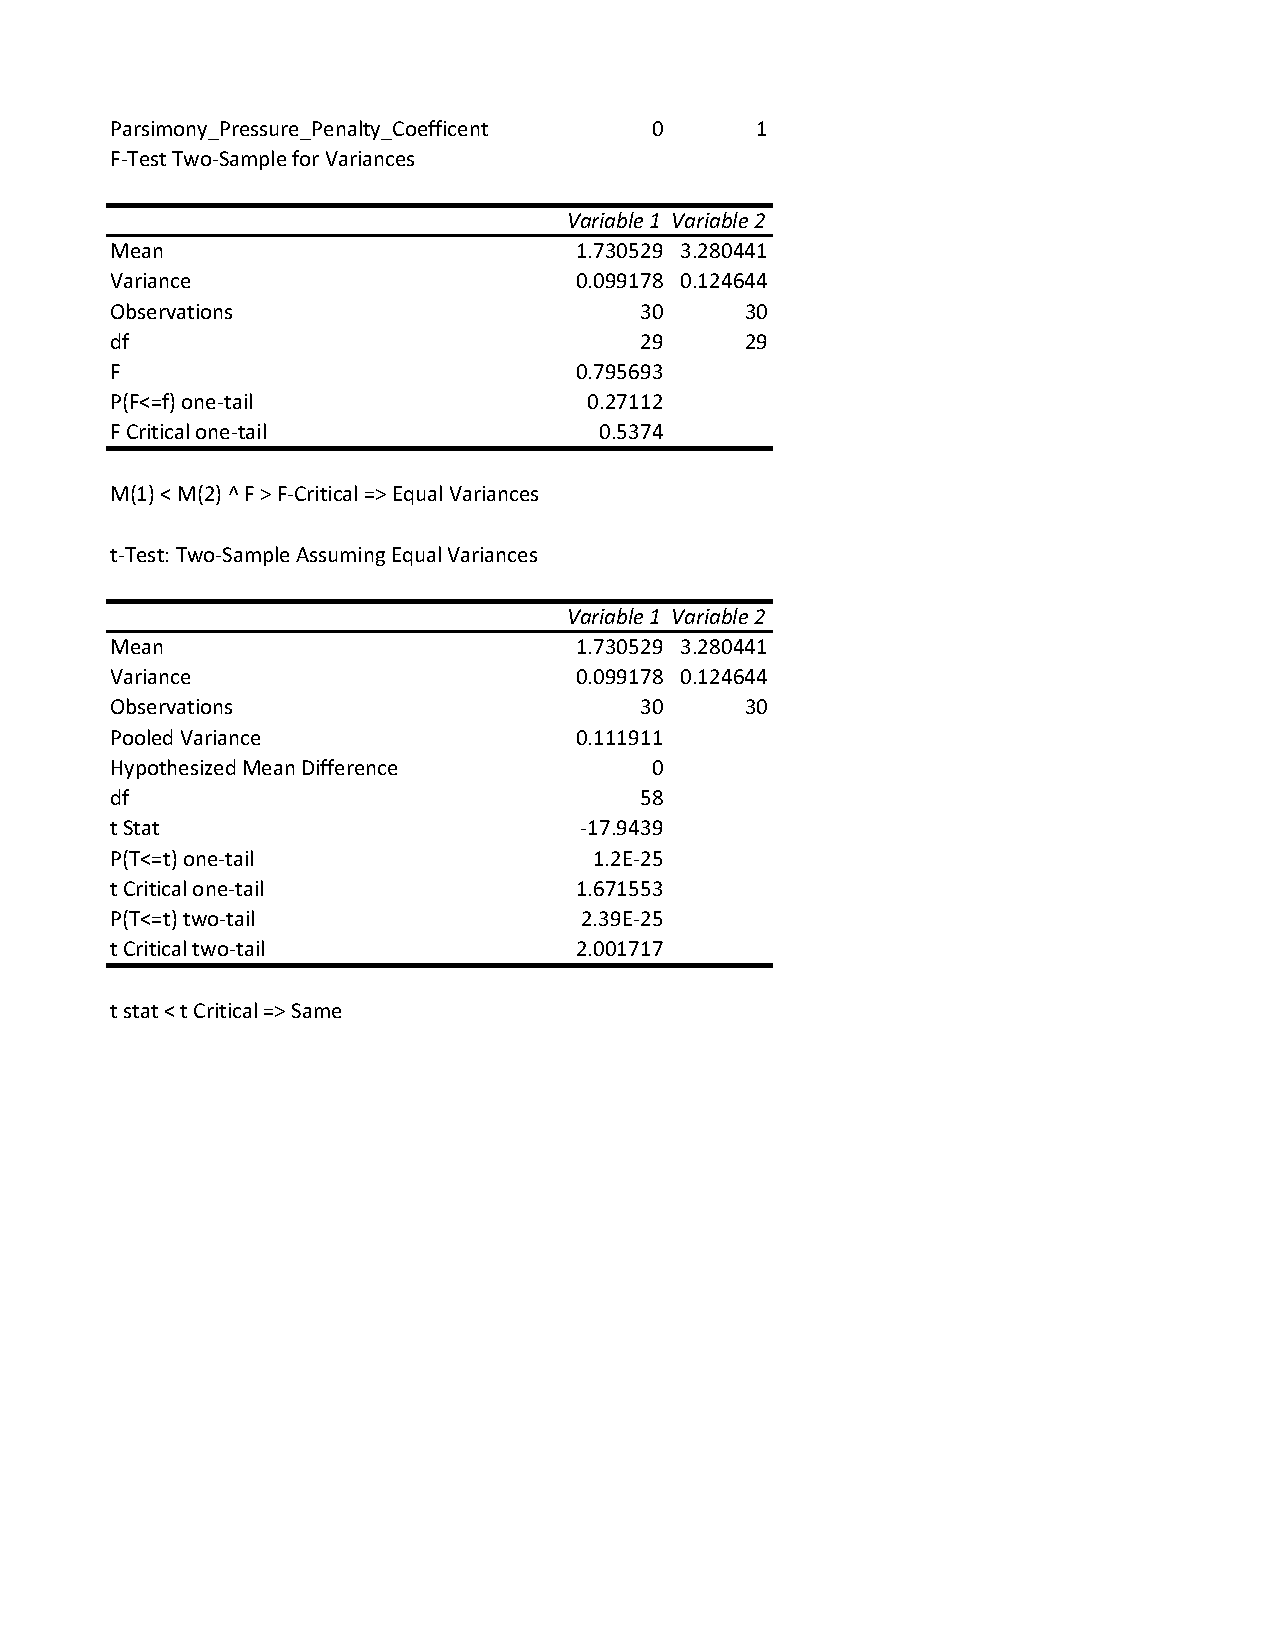
\includegraphics[width=\textwidth]{./pictures/relative_02.pdf}
	\end{figure}

	\begin{figure}
		\caption{Statistical Analysis for Relative Parsimony Pressure Penalty Coefficient 0.5 VS 1.0}
		\label{fig:stat_rel_12}
		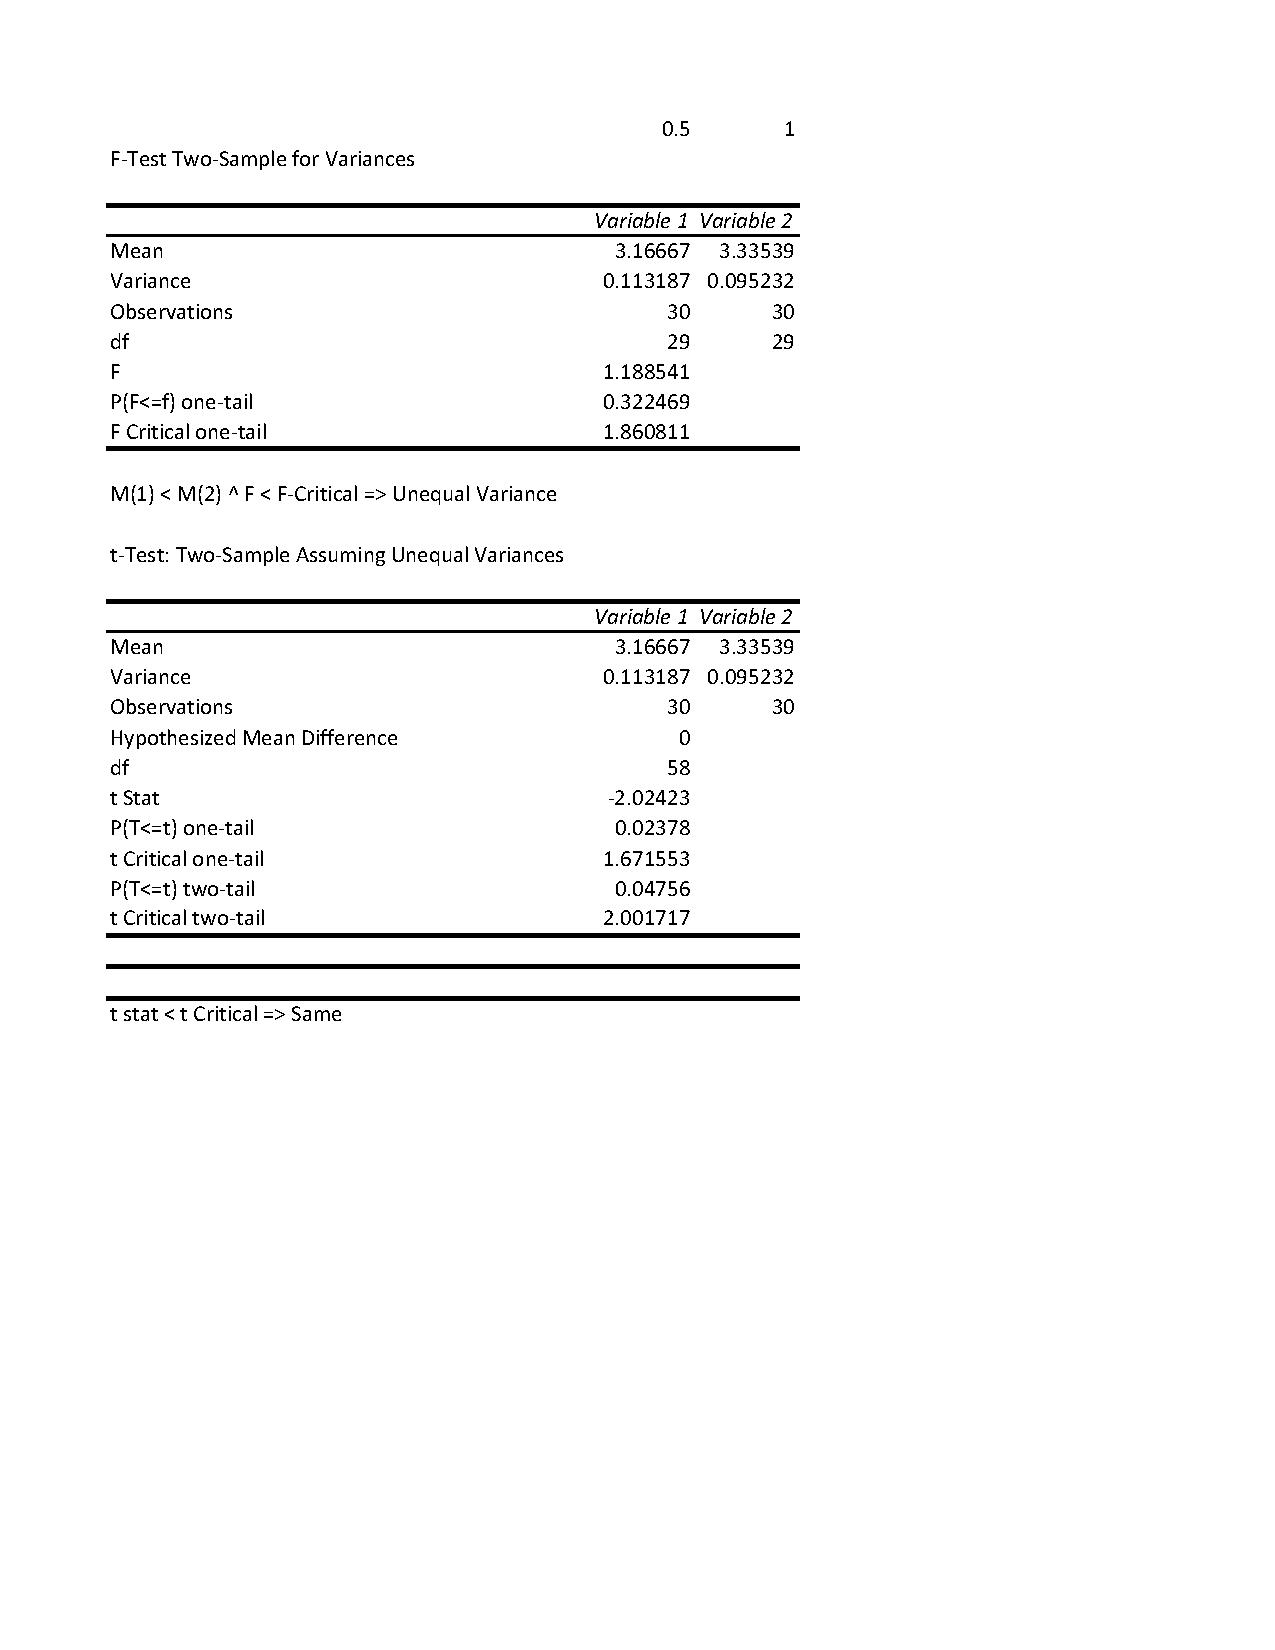
\includegraphics[width=\textwidth]{./pictures/relative_12.pdf}
	\end{figure}

	\begin{figure}
		\caption{Statistical Analysis for Absolute Parsimony Pressure Penalty Coefficient 0.0 VS 0.5 and 1.0 (NOTE: 0.5 and 1.0 have the same absolute fitness)}
		\label{fig:stat_abs_012}
		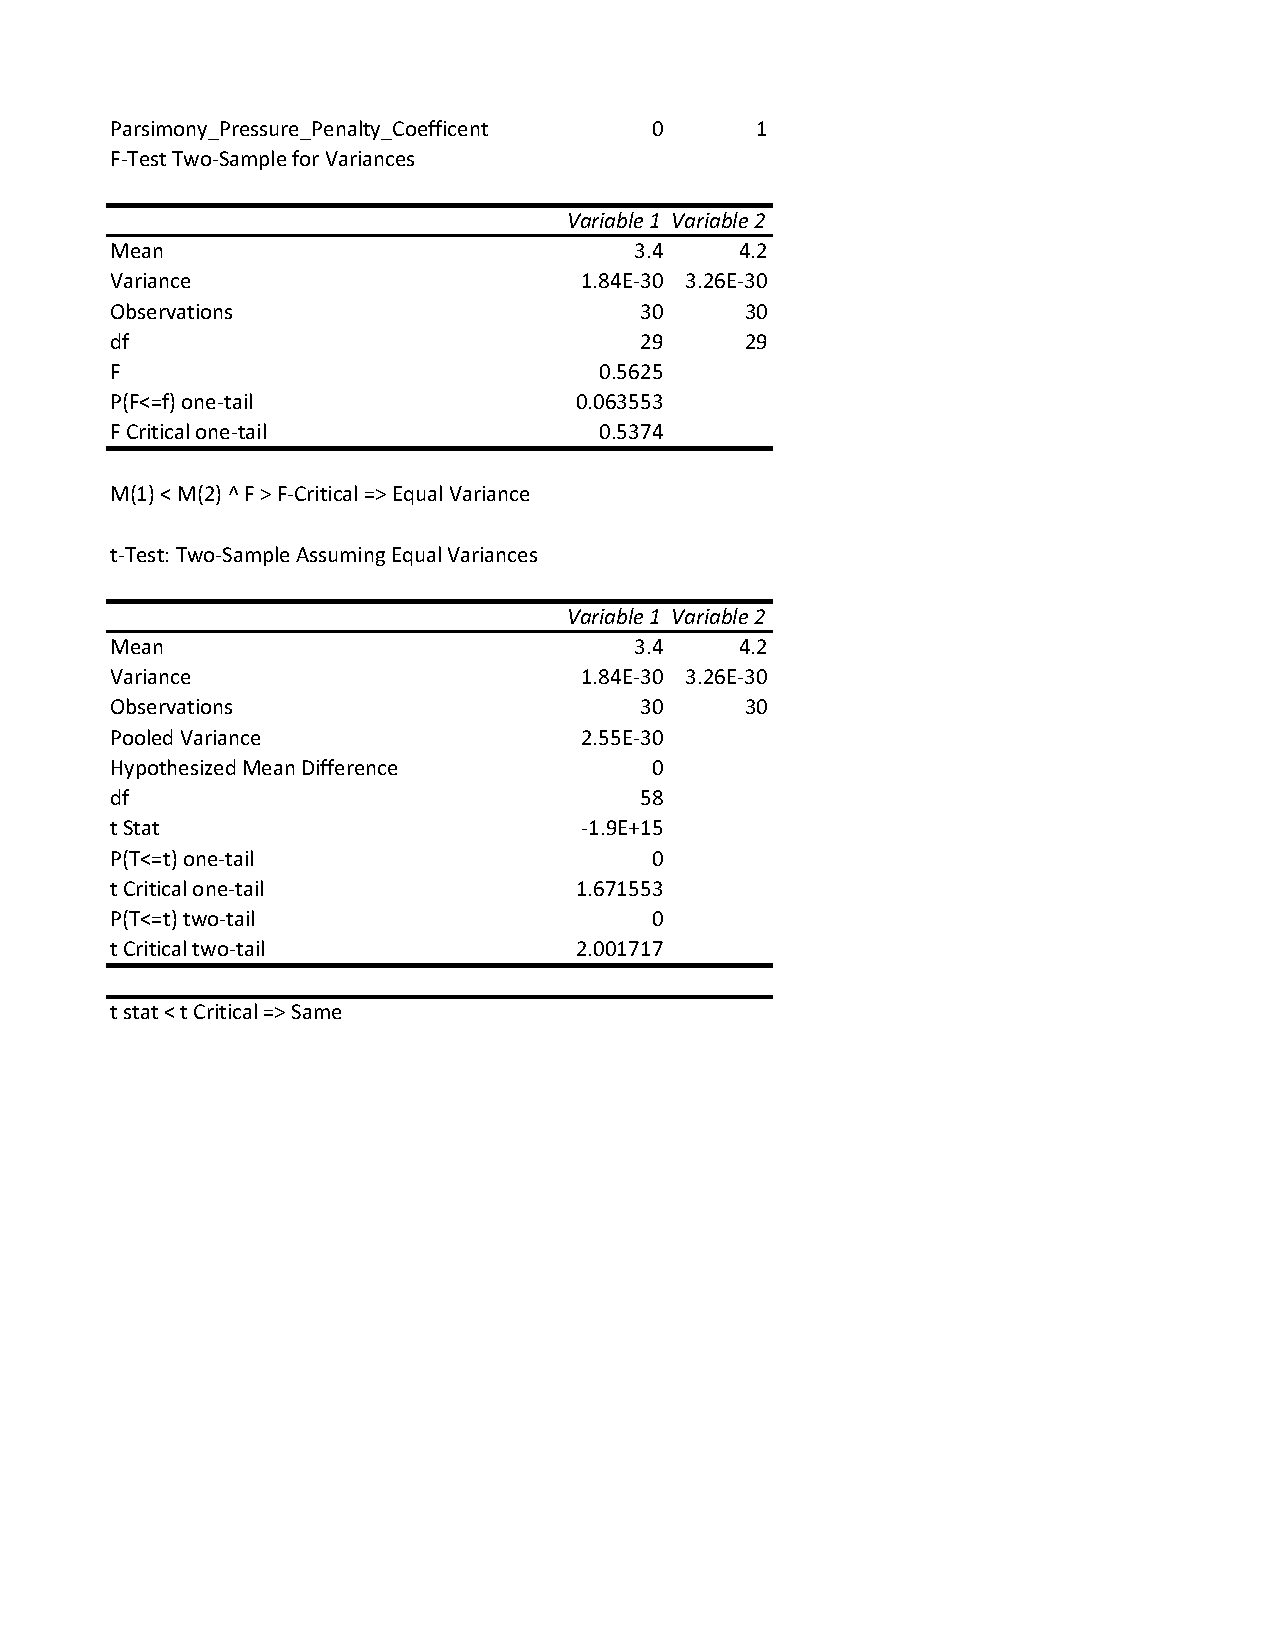
\includegraphics[width=\textwidth]{./pictures/absolute_012.pdf}
	\end{figure}

	\begin{table}
		\centering
		\caption{Averages and Standard Deviations for Each Strategy}
		\label{tab:std_mean}
		\begin{tabular}{| c | c | c |}
			\hline
									& Mean 		& Standard Deviation 	\\
			\hline
			Relative Fitness 0.0	& 1.815103267 & 0.311954147			\\
			\hline
			Relative Fitness 0.5	& 3.166669567 &	0.336432956			\\
			\hline
			Relative Fitness 1.0	& 3.335390367 &	0.308596783			\\
			\hline
			Absolute Fitness 0.0	& 2.781111167 & 0.432641637			\\
			\hline
			Absolute Fitness 0.5	& 3			 & 0					\\
			\hline
			Absolute Fitness 1.0	& 3			 & 0					\\
			\hline
		\end{tabular}
	\end{table}

	\section{Bonus 1}
	To detect cycling, a dequeue is used. Each time after survival selection is completed, the best Prisoner is added to the end of the dequeue. If this Prisoner already exists in the dequeue, but is not already at the end, then we know that cycling has occurred, as in, a Prisoner who was previously the best, but was dethroned, is now the best again. An investigation of the effects of cycling is discussed in Section \textit{Bonus 2}.

	\section{Bonus 2}
	To deter cycling, when a cycle is found, the best element is removed and replaced by a randomly generated Prisoner. This is to add diversity into the population which should prevent cycling in the future.

	In 30 runs of detecting and deterring cycling, 23 cycles were formed and deterred. As can be seen in Figure \ref{fig:rel_bonus}, average fitness slowly increases while best fitness slowly decreases, similar to its none deterring counterpart \ref{fig:relative_plot_2}. As with the main experiment, this might be due to the Prisoners getting better at playing with one another. Figure \ref{fig:abs_bonus} shows that the absolute fitness is maximized initially and stays maximized for the rest of the run, average fitness remains mostly stagnant.

	Figure \ref{fig:stat_rel_bonus} shows the relative statistics comparing trial 3 (parsimony coefficient = 1.0) to the bonus trial. It is shown that the normal trial without cycling detection is significantly better in the relative fitness case. This is probably because the best Prisoner is thrown away when a cycle is detected. However, in the absolute fitness case, both algorithms perform equally well, both performing optimally against tic-for-tat. Table \ref{tab:std_mean_bonus} shows the mean and standard deviation for the bonus trial.

	\begin{figure}
		\caption{Relative Fitness For Bonus 1 and 2}
		\label{fig:rel_bonus}
		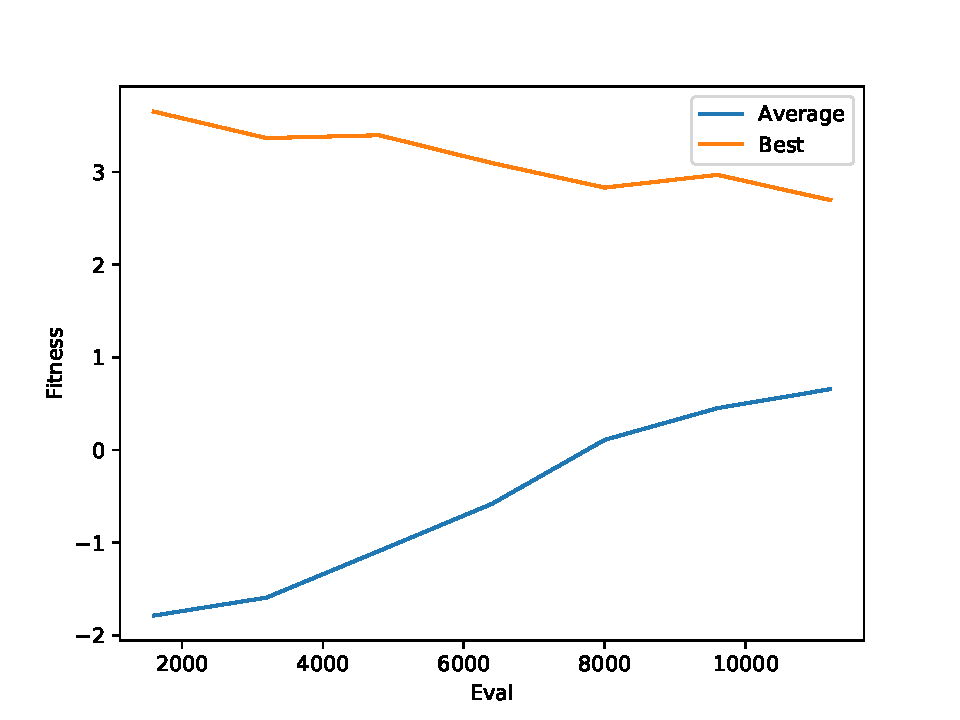
\includegraphics[width=\textwidth]{../graph/graphs/7.pdf}
	\end{figure}

	\begin{figure}
		\caption{Absolute Fitness For Bonus 1 and 2}
		\label{fig:abs_bonus}
		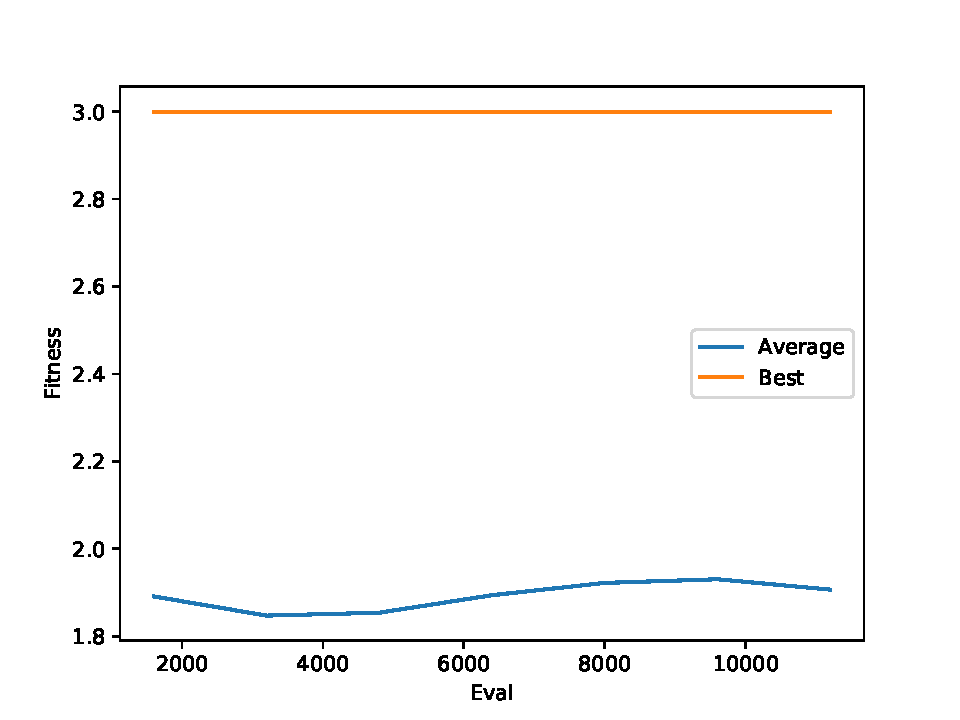
\includegraphics[width=\textwidth]{../graph/absolute/7.pdf}
	\end{figure}

	\begin{figure}
		\caption{Statistical Analysis Comparing Base Problem to Bonus 1 and 2 using Relative Fitness}
		\label{fig:stat_rel_bonus}
		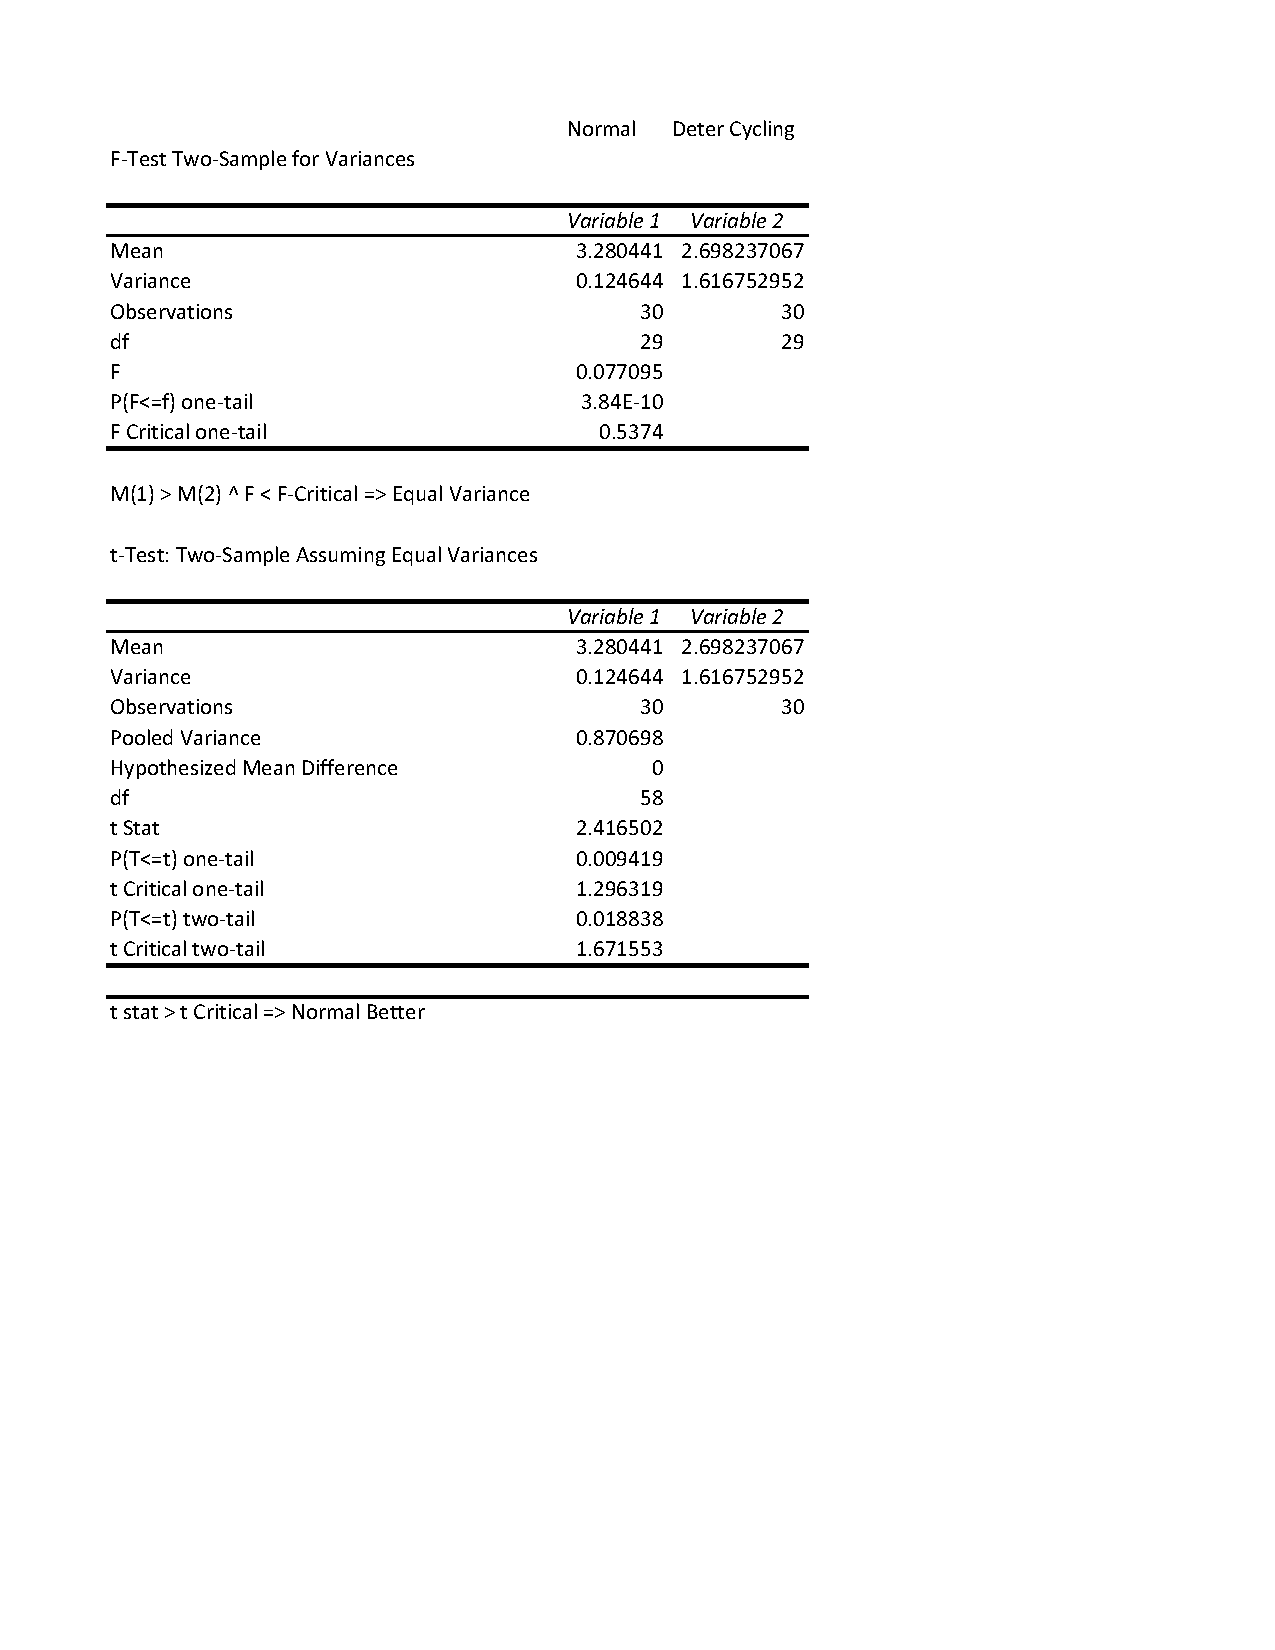
\includegraphics[width=\textwidth]{./pictures/stat_rel_bonus.pdf}
	\end{figure}

	\begin{table}
		\centering
		\caption{Averages and Standard Deviations for Bonus}
		\label{tab:std_mean_bonus}
		\begin{tabular}{| c | c | c |}
			\hline
									& Mean 		& Standard Deviation 	\\
			\hline
			Relative Fitness 1.0	& 2.697945567 & 1.27891655			\\
			\hline
			Absolute Fitness 1.0	& 3			 & 0					\\
			\hline
		\end{tabular}
	\end{table}
		
\end{document}
